\begin{figure*}[ht!]
\centering
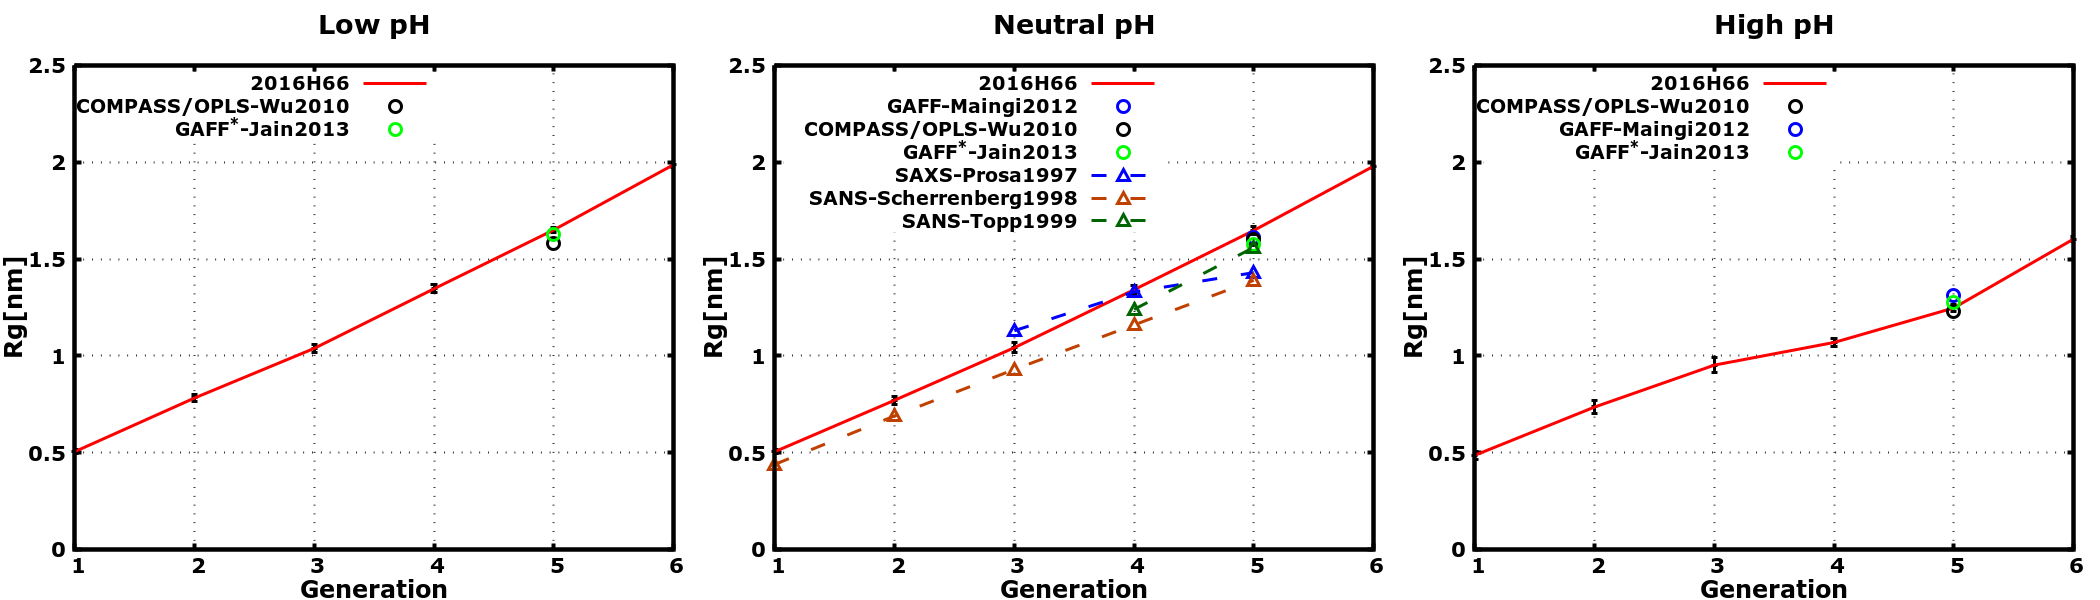
\includegraphics[width=\textwidth]{images/PME/PPIRg.png}
\caption{Raio de giro ($R_g$) em função da geração em meios de pH baixo (curva da esquerda), neutro (curva do meio) e alto (curva da direita).
Os resultados obtidos com o campo de força 2016H66\cite{Horta2016} são comparados com resultados de estudos experimentais e de simulações prévios:
Prosa1997\cite{Prosa1997}, %\cite{PR97.2},
Scherrenberg1998\cite{Scherrenberg1998}, %\cite{SC98.Y},
Topp1999\cite{Topp1999}, %\cite{TO99.Y},
Wu2010\cite{Wu2010}, %\cite{WU10.5},
Maingi2012\cite{Maingi2012}, %\cite{MA12.23},
Jain2013\cite{Jain2013}, %\cite{JA13.4}}
Smeijers2016\cite{Smeijers2016}.} %\cite{SM16.Y}
\label{supfig:PPIRg}
\end{figure*}

\begin{figure*}[ht!]
\centering
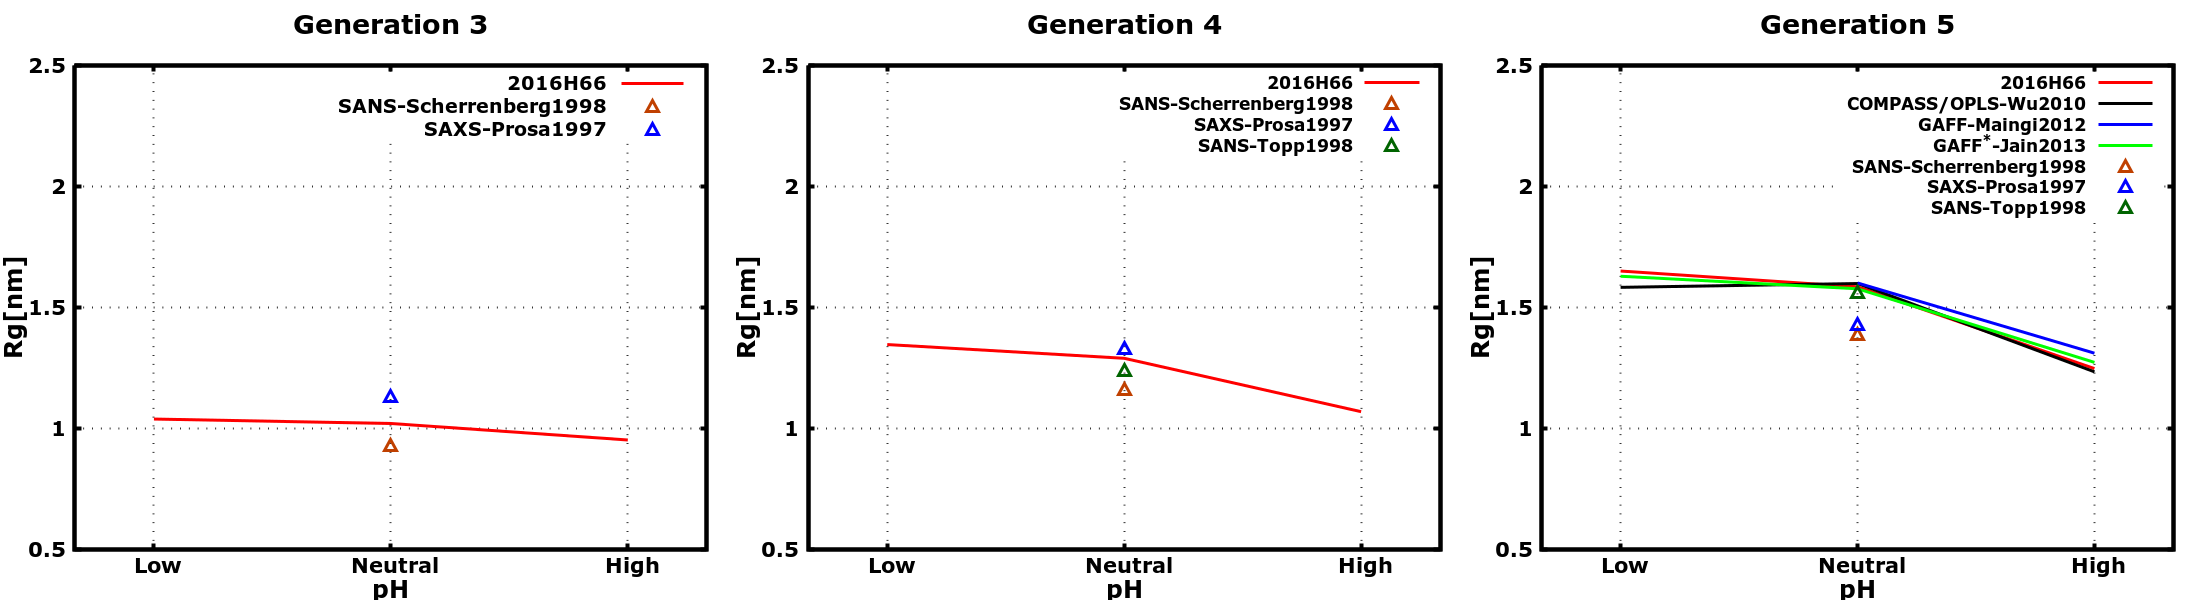
\includegraphics[width=\textwidth]{images/PME/PPIgyrateGpH.png}
\caption{Raio de giro ($R_g$) em função do pH para o PPI de geração 3 (curva da esquerda), 4 (curva do meio) e 5 (curva da direita).
Os resultados obtidos com o campo de força 2016H66\cite{Horta2016} são comparados com resultados de estudos experimentais e de simulações prévios:
Prosa1997\cite{Prosa1997}, %\cite{PR97.2},
Scherrenberg1998\cite{Scherrenberg1998}, %\cite{SC98.Y},
Topp1999\cite{Topp1999}, %\cite{TO99.Y},
Wu2010\cite{Wu2010}, %\cite{WU10.5},
Maingi2012\cite{Maingi2012}, %\cite{MA12.23},
Jain2013\cite{Jain2013}, %\cite{JA13.4}}
Smeijers2016\cite{Smeijers2016}.} %\cite{SM16.Y} and
\label{supfig:PPIRgpH}
\end{figure*}

\begin{figure*}[ht!]
\centering
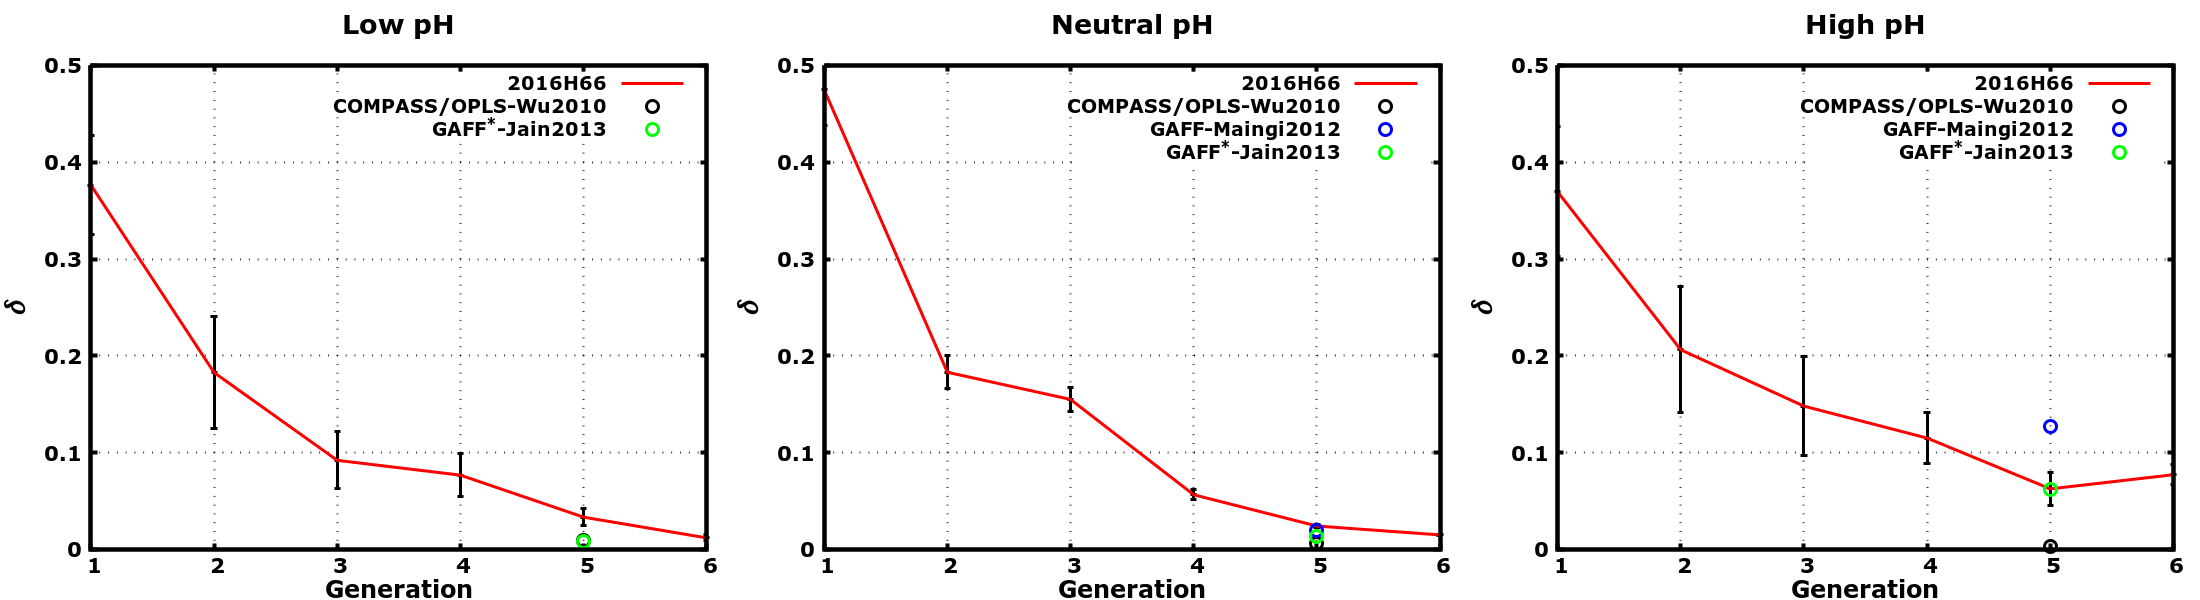
\includegraphics[width=\textwidth]{images/PME/PPIAsphericity.png}
\caption{Asfericidade $\delta$ do PPI em função da geração. As curvas da esqueda para a direita mostram os sistemas em baixo, neutro e alto pH, respectivamente.
Os resultados obtidos com o campo de força 2016H66\cite{Horta2016} são comparados com resultados de estudos experimentais e de simulações prévios:
Wu2010\cite{Wu2010}, %\cite{WU10.5}, 
Maingi2012\cite{Maingi2012}, %\cite{MA12.23}, 
Jain2013\cite{Jain2013}.} %\cite{JA13.4}}
\label{supfig:PPIAsphericity}
\end{figure*}

\begin{figure}[ht!]
\centering
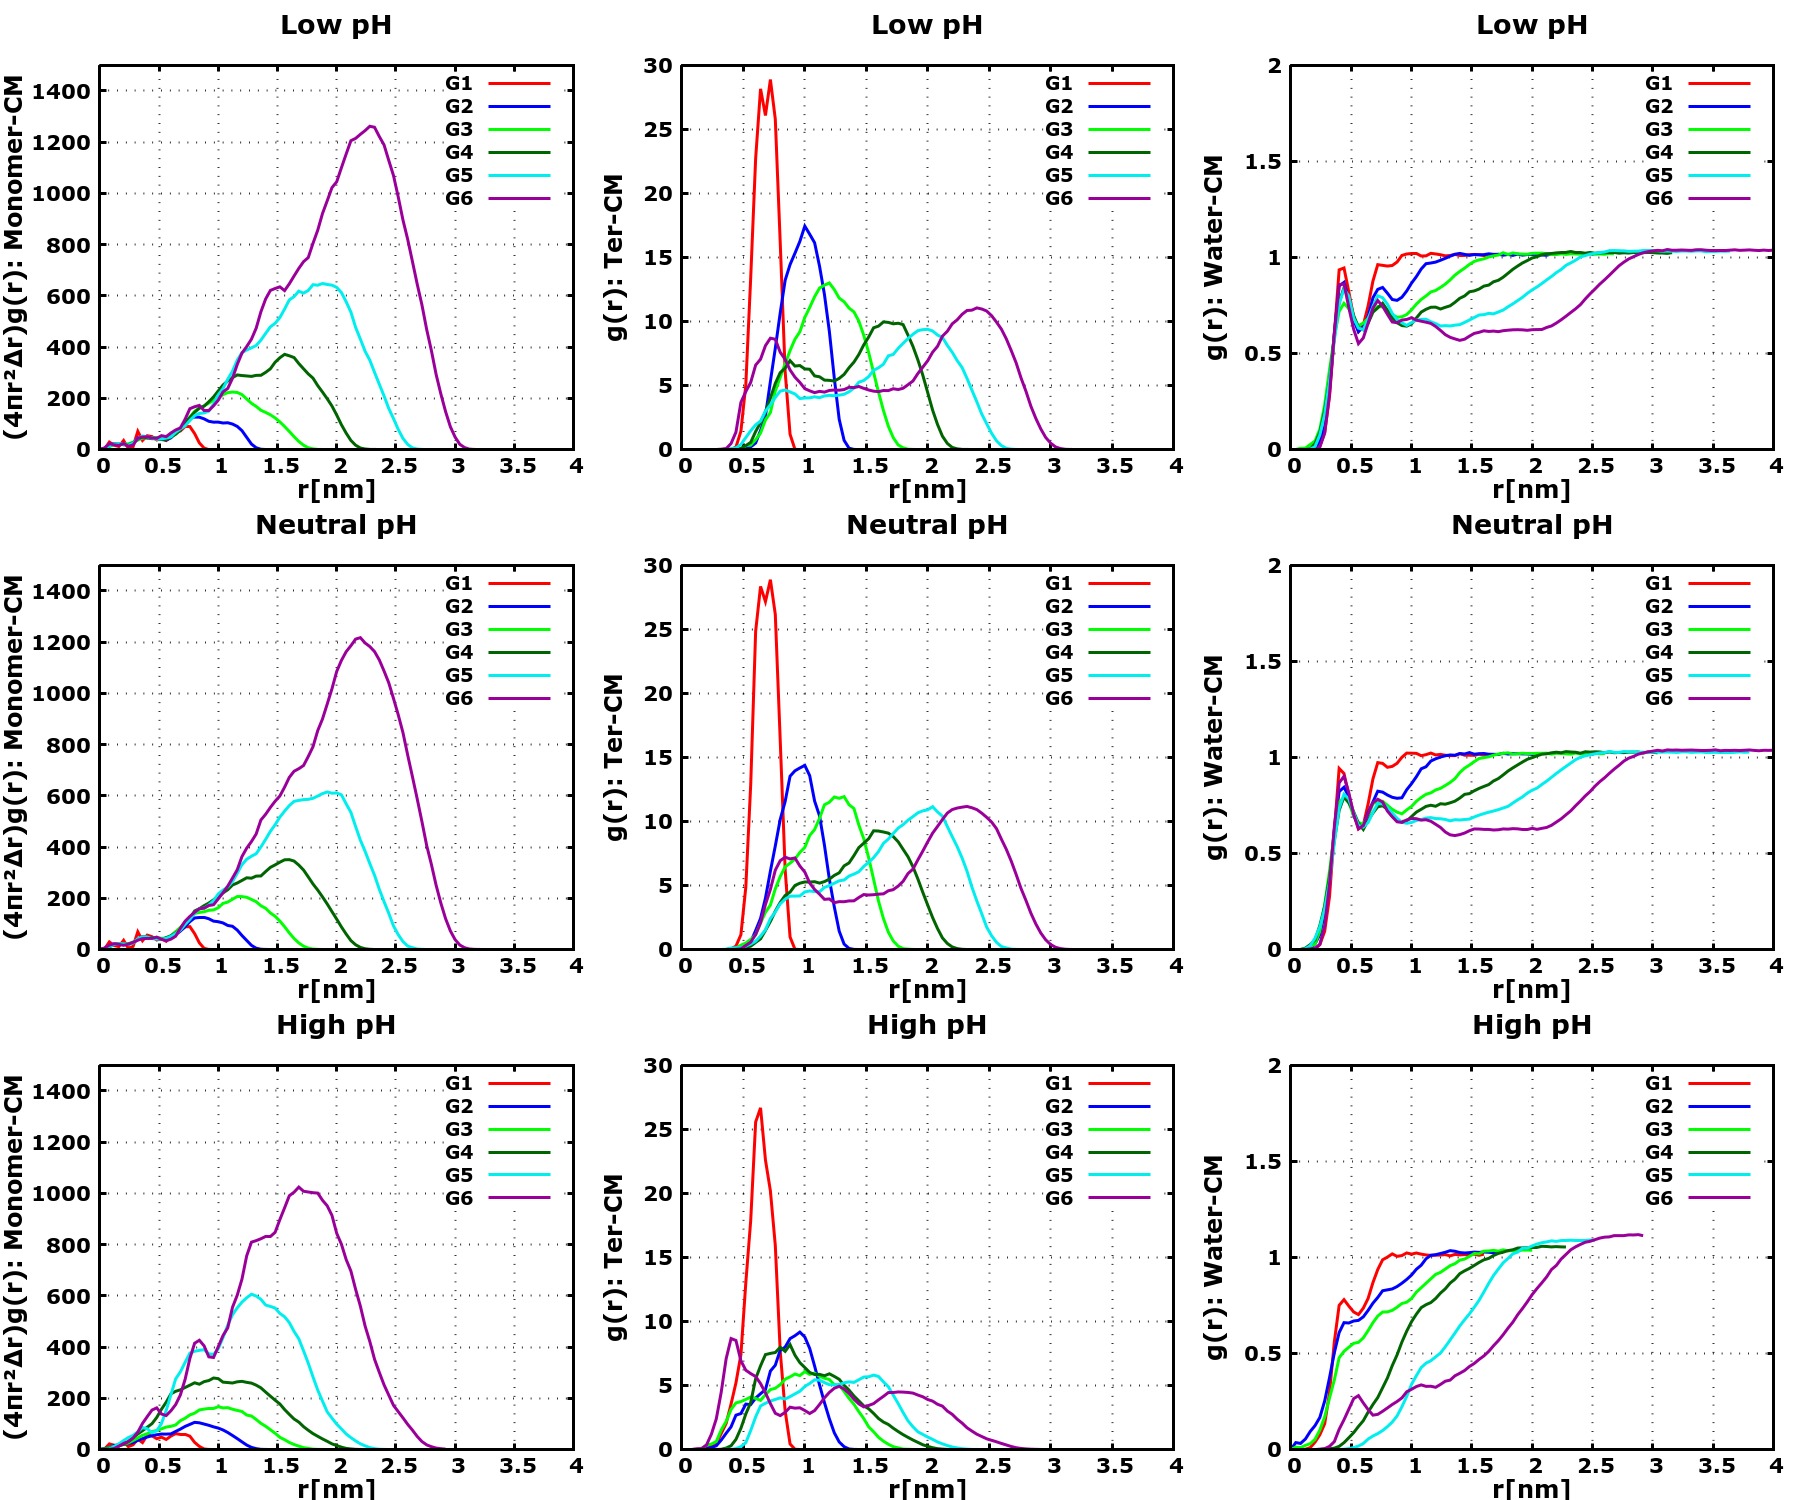
\includegraphics[width=\textwidth]{images/PME/PPIRDF.png}
\caption{Função de distribuição radial (RDF) $g(r)$ para o PAMAM. As curvas da esquerda, do meio e da direita mostram, respectivamente, as RDFs do centro de massa do dendrímero em relação à todos os átomos do dendrímero, às aminas primárias terminais e às moléculas de água. E as linhas superiores, intermediárias e inferiores mostram os RDFs descritos anteriormente em condições de pH baixo, neutro e alto, respectivamente. A coluna da esquerda não foi normalizada pelo volume da camada esférica utilizada.}
\label{supfig:PPIRDF}
\end{figure}

\begin{figure}[ht!]
\centering
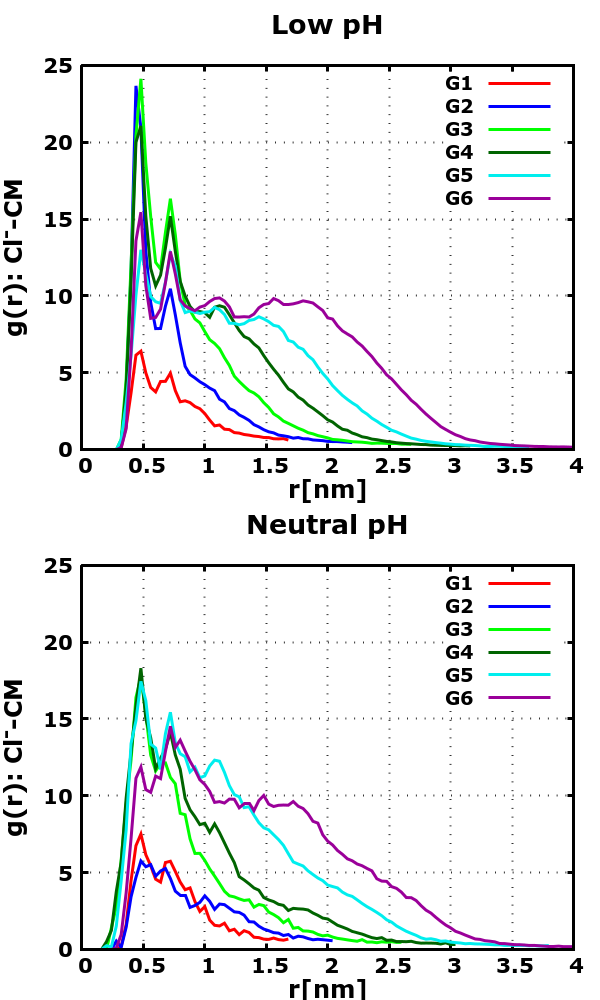
\includegraphics[scale=0.3]{images/PME/PPIClRDF.png}
\caption{Função de distribuição radial g(r) para o PPI. As curvas mostram o RDF de contra-íons cloreto em relação ao centro de massa do dendrímero para os casos onde o contra-íon está presente(pHs alto e neutro).}
\label{supfig:PPIClRDF}
\end{figure}